\section{Simulation}

A realistic model of the LTCC has been developed, describing the location and material composition
of the support box, the mirrors, PMTs, Winston-Cones, magnetic shields and the $C_4F_{10}$ gas, see \cite{gemc2019}.
A 3D view of the simulated geometry of the LTCC is shown in \F{simOverview}.


\begin{figure}
	\centering
	\includegraphics[width=0.99\columnwidth,keepaspectratio]{img/simOverview.png}
	\caption{The Geant4 model of the LTCC implemented in GEMC \cite{gemc2019}. This setup corresponds to the
             initial LTCC configuration for the first CLAS12 production running in spring 2018
			 where the LTCC sectors 2, 3, 5 and 6 were present. In this picture the hyperbolic mirrors and some magnetic shields
             in sector 3 (upper right) have been made transparent to show details of the Winston cones (grey) and magnetic shields (black).}
	\label{fig:simOverview}
\end{figure}

\subsection{Geometry}

The Cherenkov light is emitted on a small cone around the direction of the emitting particle. The polar angle of
the particles entering the LTCC can be different from the polar angle at the production vertex due
to the bending of the tracks inside the toroidal magnetic field.
Instead of having two sets of mirrors, one aligned for in-bending (toward the beamline) and one aligned for
out-bending (away from the beamline) particles, the optics of the mirrors was designed to maximize the
light collection of optical photons originating from the target (placed at the center of the CLAS12 coordinate system),
to average the cases for the two charged particles.

The mirror shapes were described mathematically by ellipsoidal and hyperbolic curves.
The ellipsoid first focal point is the target location and the second focal point was chosen
to place the mirrors as far back in the box as possible to maximize the amount of gas seen by the tracks.
The second ellipsoid focal point overlaps with the hyperbolic first focal point. The hyperbole shape was optimized to focus the light
collection on PMTs placed on the shadow of the torus magnet coil, near the LTCC box walls, see \F{mirrorMath}.


\begin{figure}
	\centering
	\includegraphics[width=0.98\columnwidth,keepaspectratio]{img/mirrorMath1.png}
	\includegraphics[width=0.98\columnwidth,keepaspectratio]{img/mirrorMath2.png}
	\caption{The geometry of the LTCC mirrors is defined my the mathematical equations of the ellipse and hyperbola.
             Top: the ellipsoidal curve (solid line), with its center (square) and its focal points
             (circle at the origin, representing the target, and the bottom star).
             The two hyperbolas curves, defined by the two focal points (stars, one coinciding with the ellipse
			 focal point and the other at the desired location of the PMT) are the dashed lines. The
			 hyperbola at the bottom is the one that define the hyperbolic mirror.
             Bottom: zoomed in details of the setup above. The squares represent the mirrors left and right edges.
             These parameters are stored in databases and loaded in the software modeling the LTCC mirrors
             in the GEMC simulation \cite{gemc2019}.}
	\label{fig:mirrorMath}
\end{figure}

In the Geant4 implementation the elliptical mirrors are produced in three steps, each a boolean operation of volumes:

\begin{enumerate}
	\item make ellipsoidal mirror shells: by subtracting of two ellipsoidal volumes, rotated and centered on their designed position.
	\item cut out the mirrors from the shells: subtraction of the shells with left, right, top, and bottom boxes.
	\item place cut out mirrors: rotate and place the mirrors in the final position within the LTCC mother volume.
\end{enumerate}

The hyperbolic mirrors are made by Geant4 ``polycons'' that approximate the shape of the mirrors using a number of facets
varying from 10 (smallest mirror) to 30 (longest mirrors). The measured reflectivity is included in the simulation as
an optical property of the mirror material.

The CAD engineering models of the WCs have been used in the simulations, see \F{wcSimulation}.
The measured reflectivity is included in the simulation as an optical property of the WC material.
The WC and the PMT volumes are surrounded by boxes of mu-metal that model the LTCC magnetic shields, see \F{simShield}.

\begin{figure}
	\centering
	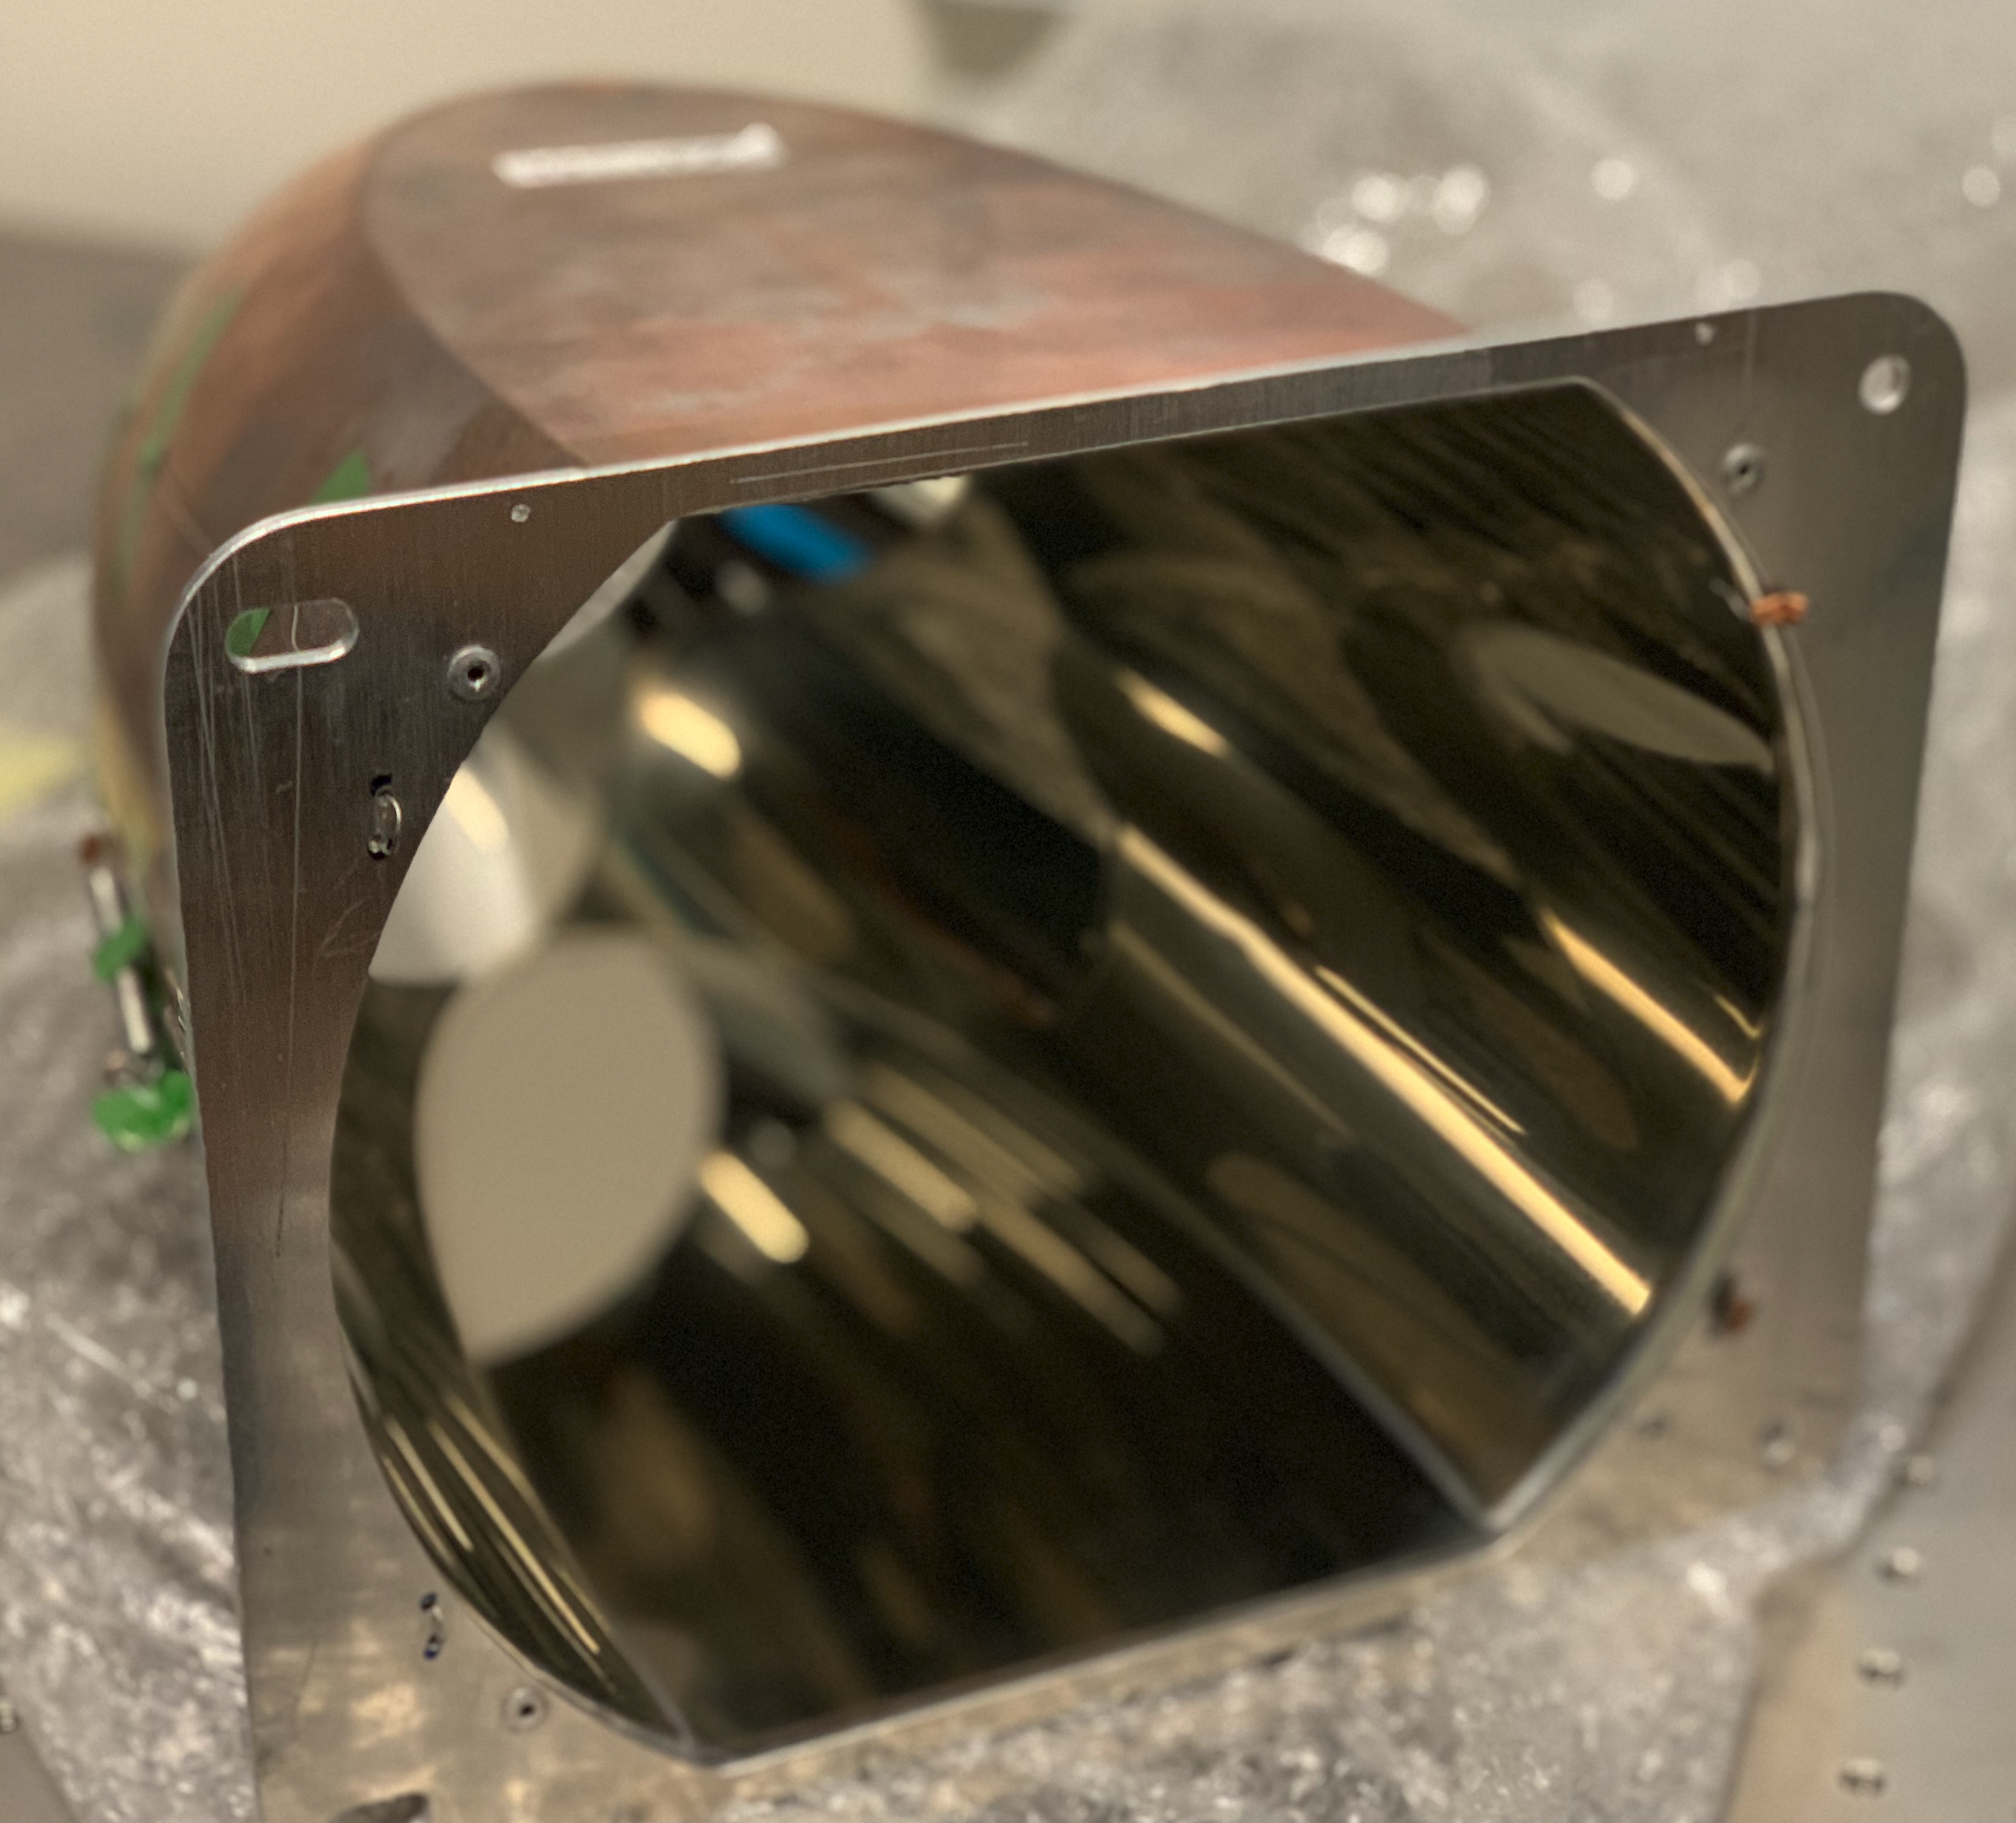
\includegraphics[width=0.99\columnwidth,keepaspectratio]{img/wcLargeReal.png}
	\includegraphics[width=0.99\columnwidth,keepaspectratio]{img/wcLargeSim.png}
	\caption{Top: a photograph of the large WC used for segments 12 to 18. Bottom: the tessellated volume used in the
            simulation, imported from the CAD engineering model.}
	\label{fig:wcSimulation}
\end{figure}

\begin{figure}
	\centering
	\includegraphics[width=0.99\columnwidth,keepaspectratio]{img/simShield.png}
	\caption{The magnetic shields are modeled by mu-metal boxes in the GEMC simulations (black). The WC (grey) focus the light on the red PMT surface.}
	\label{fig:simShield}
\end{figure}


The LTCC box support structure was imported from the engineering model shown in \F{boxCut}. This includes the 1-cm thick aluminum
elliptical and hyperbolic mirror support flanges, the nose, and the hardware mount to the CLAS12 beamline.


\subsection{Digitization}

In the digitization the number of collected photons is converted to charge by taking into account:

\begin{itemize}
	\item The quantum efficiency of the PMTs
	\item The position and width of the single photo-electron peak as stored in the CLAS12 calibration database
\end{itemize}


\subsection{Run Period Variations}

As the start of CLAS12 beam operations, there was not sufficient $C_4F_{10}$ gas to fill all sectors, so some LTCC sectors
where removed from the Forward Carriage. As they were installed or removed, any gas leaks were found and fixed.
These CLAS12 configuration changes are imported in GEMC as database variations of the simulation setup.
The default simulations only include sector 2 (S2), S3, S5, and S6 as the RICH detector replaces the LTCC S1 and S4.
The variations are listed in Table \ref{tab:simVariations}.

\begin{table}
	\begin{center}
		\begin{tabular}{| l | c |}
			\hline \hline
			Run Period       & Sectors Installed and Gas \\
			\hline
			Default          & S2, S3, S5, S6, all $C_4F_{10}$    \\
			RGA Spring 2018  & S2, S3, S6 (N$_2$), S5 ($C_4F_{10}$)  \\
			RGA Fall 2018    & S3 ($C_4F_{10}$), S5 (N$_2$)          \\
			RGB Spring 2018  & S3 ($C_4F_{10}$), S5 ($C_4F_{10}$) \\
			\hline \hline
		\end{tabular}
	\end{center}
	\caption{LTCC simulation variations for different CLAS12 run periods. Shown are which sectors are present and the gas in each sector}
	\label{tab:simVariations}
\end{table}






